\newpage

\section*{ $^{48}$Ti(n,p)$^{48}$Sc }

Power Level: 100 kW(th) \\
Time at Power: 60.0 m \\
Wait Time: 60.0 m \\
Counting Time: 30.0 m \\
Total Activity at Removal: 2.92e-02 $\mu Ci$

\begin{table*}[h]
\centering
\begin{tabular}{ |c|c|c|c|c|c| }
 \hline
 Position & Mass $mg$ & Counting Activity $\mu Ci$ & Area (Counts) & Error \% \\
 \hline 
 1 & 5.50 & 7.19e-03 & 1.13e+04 & 0.9423 \\ 
\hline
 2 & 5.10 & 1.01e-02 & 1.58e+04 & 0.7966 \\ 
\hline
 3 & 5.10 & 7.93e-03 & 1.24e+04 & 0.8972 \\ 
\hline
 4 & 5.30 & 3.77e-03 & 5.90e+03 & 1.3019 \\ 
\hline
\end{tabular}
\end{table*}

\begin{figure}[h]
\centering
\begin{subfigure}{.5\textwidth}
  \centering
     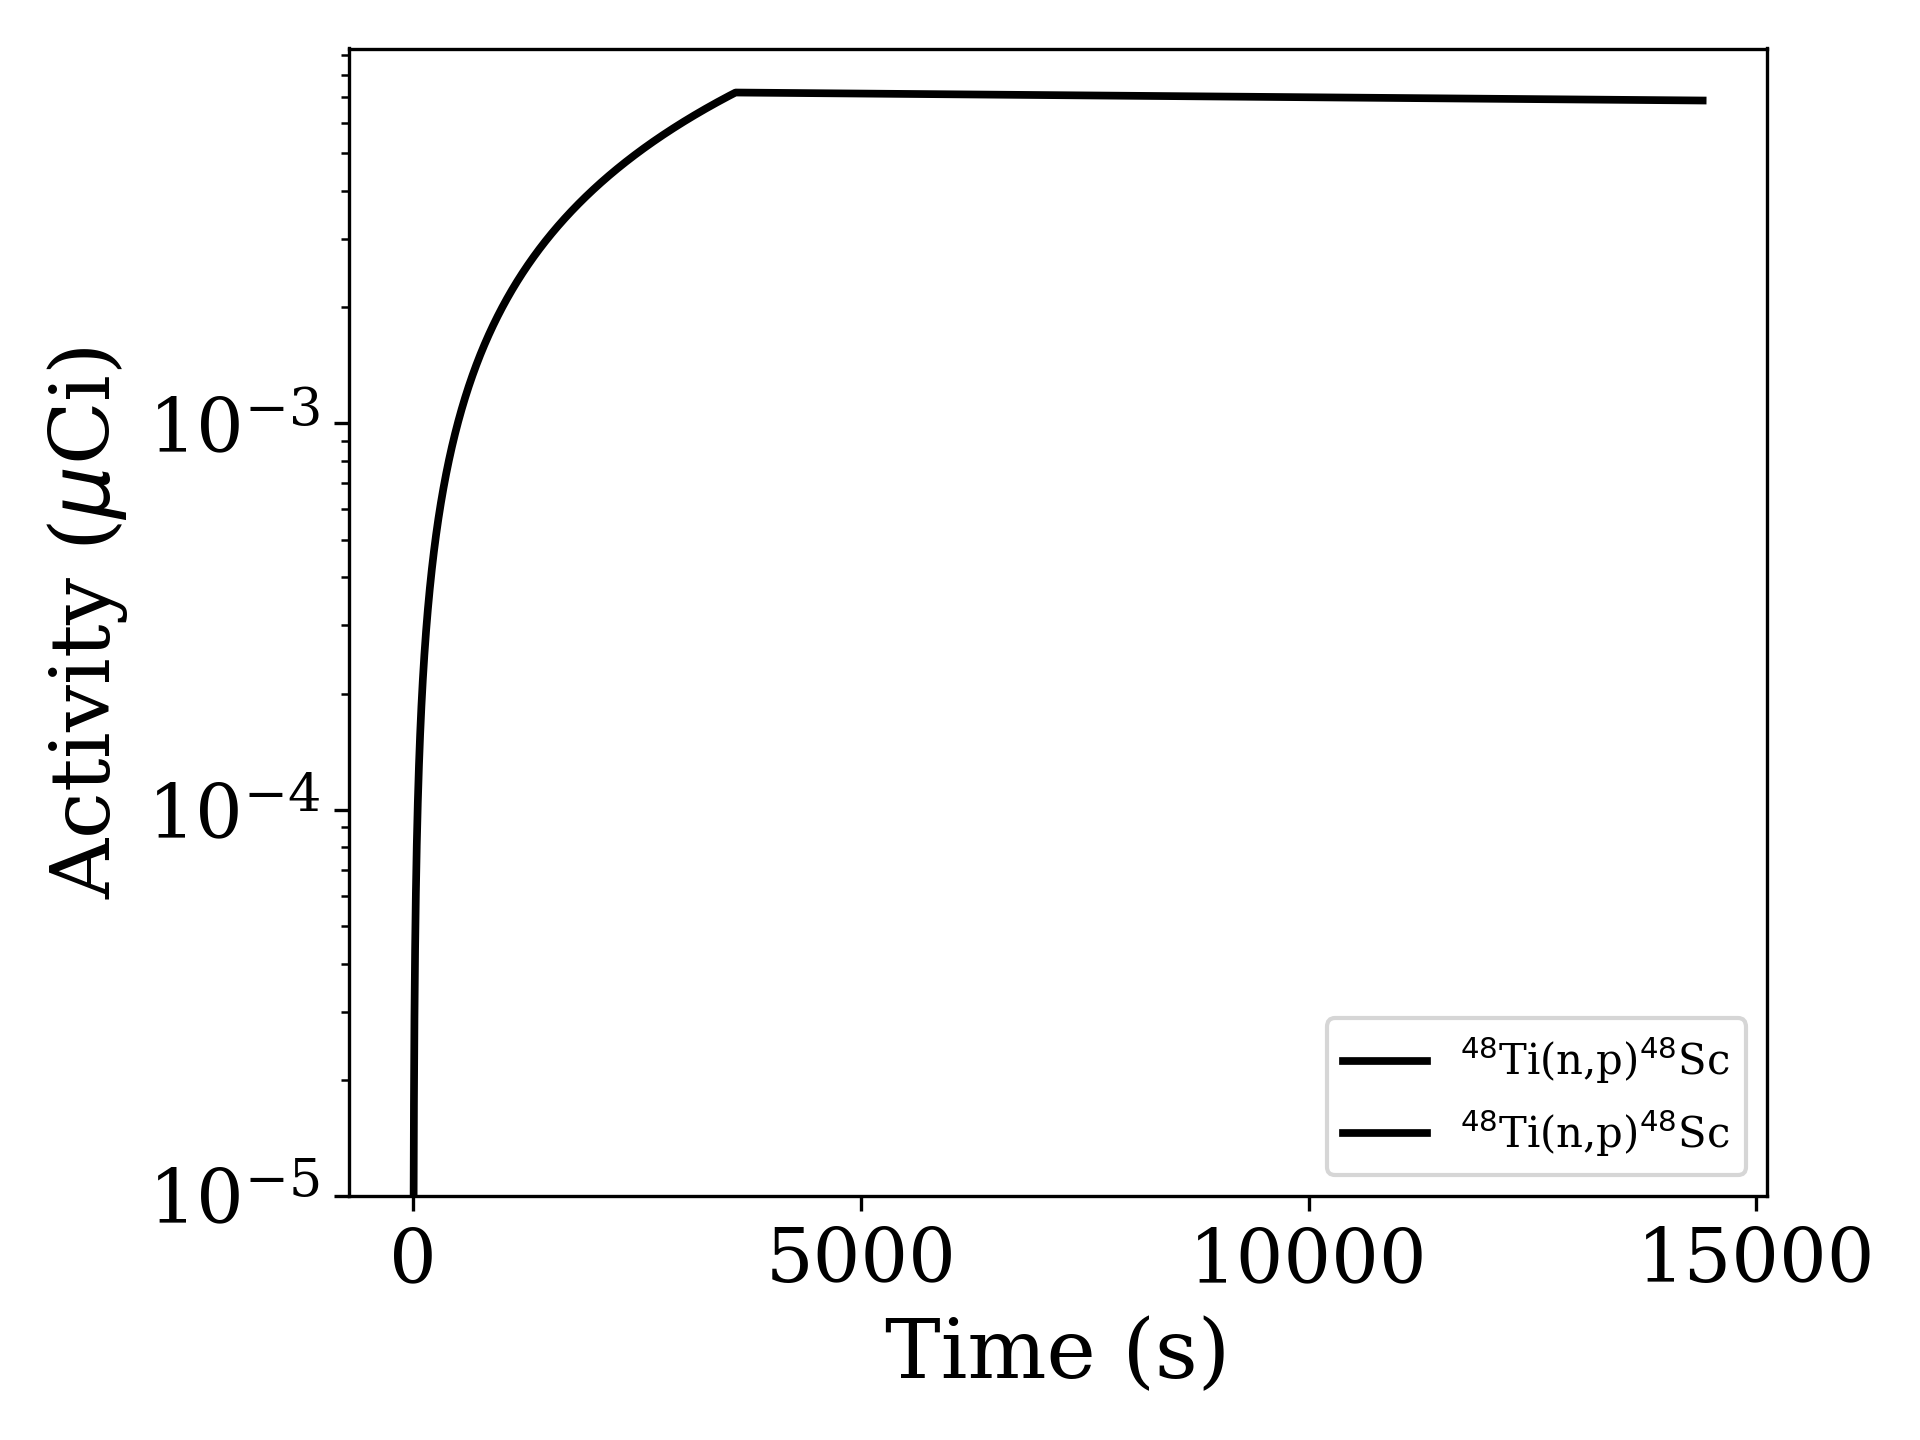
\includegraphics[width=.8\textwidth]{plot/Ti-48(n,p)Sc-48_wisconsin1} 

  \caption{Activity}
\end{subfigure}%
\begin{subfigure}{.5\textwidth}
  \centering
     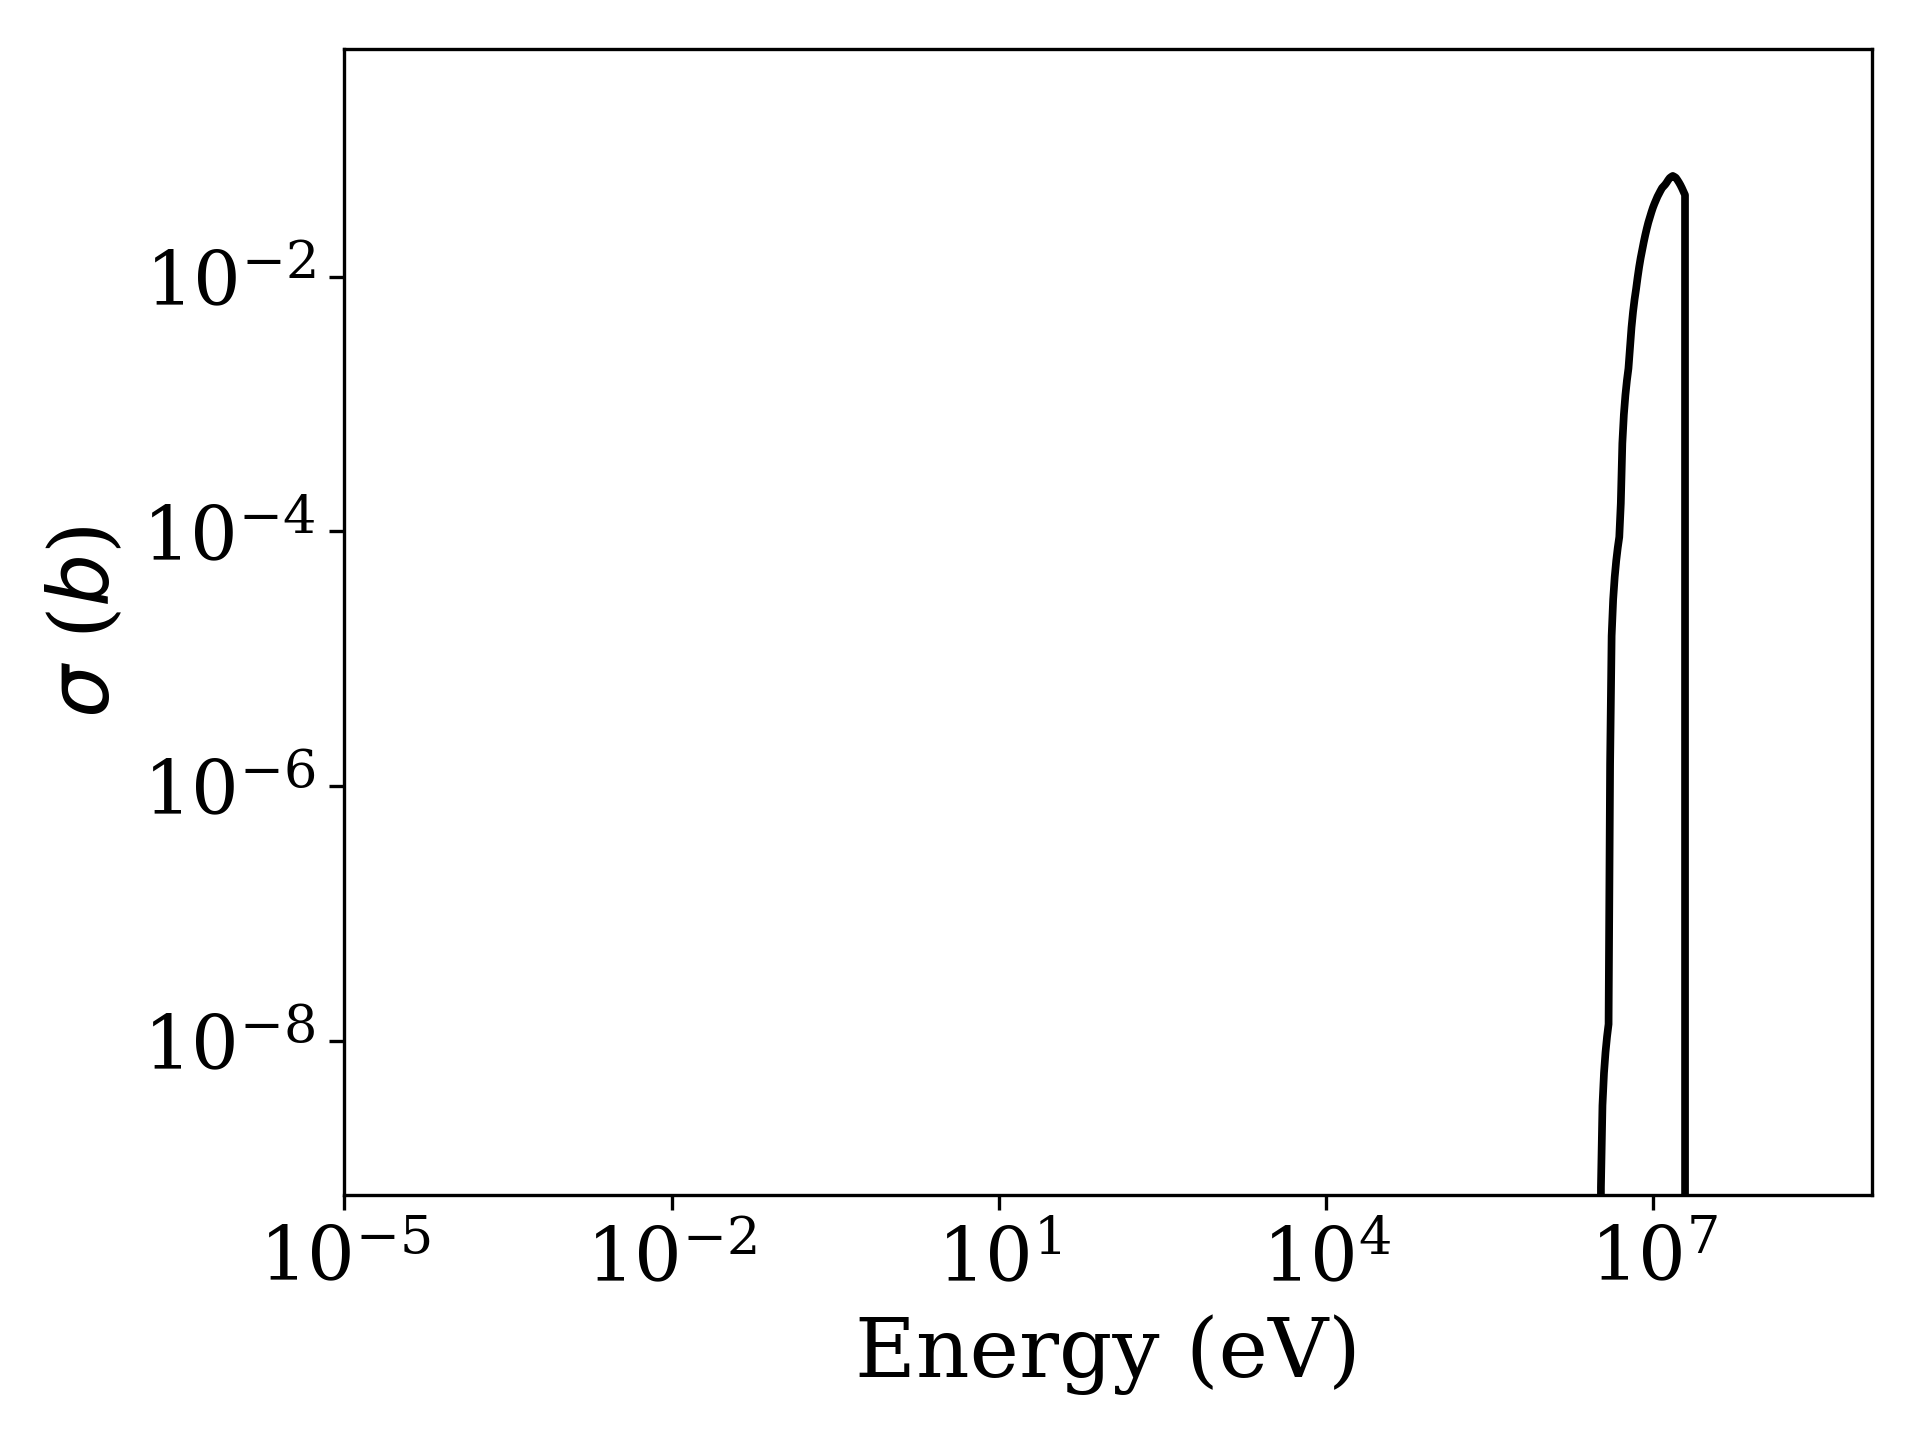
\includegraphics[width=.8\textwidth]{plot/Ti-48(n,p)Sc-48} 

  \caption{Cross Section}
\end{subfigure}
\end{figure}

\begin{table*}[h]
\centering
\begin{tabular}{ |c|c|c|c|c|c|c| }
 \hline
 Reaction & T$_{1/2}$ & ROI (eV) & Important Gammas (keV) \\
 \hline 
 $^{48}$Ti(n,p)$^{48}$Sc &  1.8 d & 5.81e+06, 1.20e+07 & 983(1.0) \\ 
\hline
\end{tabular}
\end{table*}
